\section{Computação Quântica} 
\label{quantum_comp}

A computação quântica é uma abordagem inovadora quando se trata de processamento de dados na computação. Neste capítulo é apresentado uma breve recuperação da história da área, assim bem como seus conceitos basilares e até mesmo os previstos impactos que acompanharão a funcionalidade desta inovação. Ainda, estudos adicionais estão sendo feitos a fim de complementar o capítulo para a entrega do relatório final.

\subsection{História}
Como proposto pelo cronograma desse estudo\footnote{página \pageref{updated_timeline} tabela \ref{updated_timeline}}, o presente capítulo, a ser desenvolvido no decorrer do segundo semestre, adentrará o desenvolvimento da Computação Quântica assim como a descrição de sua arquitetura – tema de extrema atualidade. O capítulo partirá do estudo de Alexander Holevo, publicado em 1973, que obteve como resultado o conhecido "teorema de Holevo"\footnote{um importante teorema limitativo na computação quântica, um campo interdisciplinar da física e da ciência da computação. Às vezes chamado de limite de Holevo, uma vez que estabelece um limite superior para a quantidade de informação que pode ser conhecida sobre um estado quântico.} – marco da computação quântica –, perpassando pela sua história até os dias atuais. Assim, poderemos compreender as implicações dos avanços em relação aos computadores quânticos, que como mencionado pelo artigo “Google claims its quantum computer can do the impossible in 200 seconds” \cite{16} já consegue resolver um problema, que levaria 10.000 anos para ser solucionado pelo supercomputador (clássico) mais rápido do mundo, em 200 segundos.

A Computação Quântica apresenta um novo horizonte de possibilidades no âmbito da computação. Acredita-se que os computadores quânticos sejam capazes de resolver certos problemas computacionais, como a factoração de inteiros – que é a base da criptografia RSA assunto aprofundado no capitulo \ref{criptography} –, substancialmente mais rápido do que os computadores clássicos.

A abordagem da computação quântica em relação à computação clássica se refere a como os dados são representados. Enquanto na computação clássica cara bit é um estado possível entre ``0'' e ``1'', já na computação quântica essa representação é probabilística, onde o dado pode estar em ambos estados ao mesmo tempo. Esse comportamento permite uma nova forma de nomear o bit, o \textbf{qubit}.

\subsection{Qubits}
\label{qubits}
Na mecânica quântica, uma partícula pode assumir dois estados ao mesmo tempo, o que é chamado de superposição. Ao aplicar este conceito à computação, temos uma partícula como um bit \footnote{melhor explicado na página \pageref{bits}} quântico, qubit (um bit quântico, unidade básica de informação em um computador quântico) que poderia retornar três posições: ligado (1), desligado (0), ou uma superposição de ambos, 1 e 0. Assim, um qubit pode comportar dois valores de uma vez; dois qubits quatro valores; e assim por diante. Isso significa que uma quantidade pequena de átomos pode comportar valores muito maiores do que os transístores de um computador binário, sendo mais eficiente. Um exemplo disto, seria o computador quântico da Google, que segundo WHYTE \cite{20}, realizou um cálculo de um problema em 200 segundos, que poderia demorar cerca de 10.000 anos para ser resolvido pelo melhor supercomputador existente, alcançando assim, a supremacia quântica.

\vspace{1cm}
\begin{figure}[H] \centering 
  \makebox[\textwidth][c]{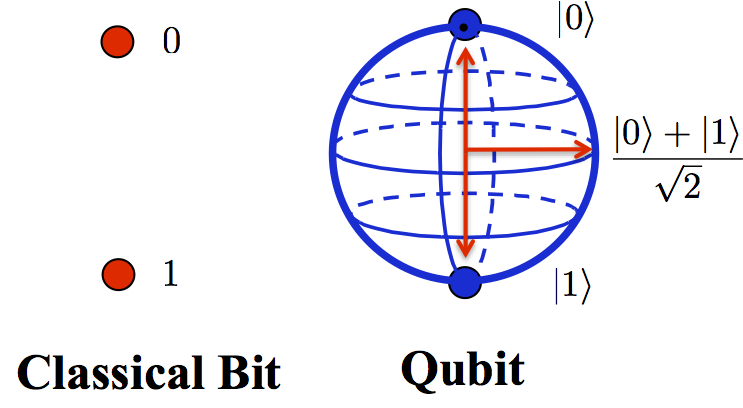
\includegraphics[width=0.5\textwidth]{bit_vs_qubit.png}}
  \caption{\label{bit_vs_qubit} A quantidade ilimitada de estados em que um qubit pode estar em um determinado momento é tradicionalmente representada em uma esfera onde Norte = 1 e Sul = 0. \href{https://www.autodesk.com}{autodesk.com}} 
\end{figure}

\subsection{Implementações}
Desde a década de 2000 as grandes empresas da computação vem se enfrentando na corrida por atingir a melhor arquitetura quântica funcional. Entre elas, destaca-se as duas grandes referencias no mercado da tecnologia: Google e IBM. Em 2019 a Google anunciou que havia atingido supremacia quântica como visto através do artigo: ``Quantum supremacy using a programmable superconducting processor'', \cite{17} coloca toda a sociedade às portas de um novo mundo, pois com esse poder computacional, problemas de otimização, que até então jamais seriam solucionados em tempo hábil, agora, estariam resolvidos em períodos mínimos de tempo.

Já a IBM, vem traçando a sua trajetória quântica desde 2016, lançando em maio de 2016 o IBM Q Experience, que continha um processador quântico de cinco qubit e um simulador de correspondência. Essa arquitetura, possibilitou que os usuários só interagissem por meio do compositor quântico, com um conjunto limitado de interações de dois qubit e um guia do usuário que assumiu experiência em álgebra linear. Em 2018 essa experiência teve significantes avanços, como exposto por Yuanhao Wang em seu artigo ``16-qubit IBM universal quantum computer can be fully entangled'', ``Os dispositivos backend atuais, da IBM incluem dois processadores com 5 qubits supercondutores sendo eles o ibmqx2 e o ibmqx4, um processador de 16 qubit, ibmqx5 e um processador de 20 qubit QS1\_1.'' \cite{18}, um grande avanço em apenas 4 anos. Atualmente, a empresa já vislumbra horizontes que pareciam muito distantes, anunciando que em 2023 terá um computador e David Nield – jornalista que escreve sobre ciência e tecnologia há mais de 20 anos tendo artigos publicados na Wired, Popular Science, The Guardian e Gizmodo – acredita que ``Com o IBM Quantum Condor planejado para 2023 - executando 1121 qubits, para ser exato - devemos começar a ver os computadores quânticos começarem a lidar com um número substancial de cálculos genuínos do mundo real, em vez de ficarem restritos a experimentos de laboratório.'' \cite{19}

\subsection{Dificuldades}
Apesar do avanços trazidos anteriormente, existem quatro principais dificuldades que impossibilitam o desenvolvimento e a escala de computadores quânticos no cenário atual: a qualidade do Qubit; implementação de algoritmos de correção de erros; o controle dos Qubits; e a grande quantidade de fios presentes na arquitetura.
Em relação à qualidade dos Qubits, a comunidade de estudiosos da computação quântica ainda não conseguiu chegar a um Qubit capaz de gerar instruções úteis em grande escala. Atualmente os poucos qubits nos computadores quânticos baseados em nuvem não são bons o suficiente para sistemas de grande escala,gerando erros ao executar operações entre dois qubits a uma taxa muito maior do que o necessário para se calcular com eficácia. Assim, após um certo número de instruções ou operações, os qubits atuaisproduzem uma resposta errada quando executamos cálculos, tendo a possibilidade do resultado obtido  ser indistinguível do ruído.
Uma vez que os qubits não são bons o suficiente para a escala em que precisamos que eles operem, precisamos implementar algoritmos de correção de erros que verifiquem e corrijam os erros de qubit aleatórios à medida que ocorrem. Esses são conjuntos de instruções complexos que utilizam muitos qubits físicos para estender efetivamente o tempo de vida das informações no sistema. A correção de erros ainda não foi comprovada em escala para a computação quântica, mas é uma área prioritária de pesquisa, a qual é considerada pré-requisito para um sistema quântico comercial em escala real.
Controle de Qubit: Para implementar algoritmos complexos, incluindo esquemas de correção de erros, é necessário provar a possibilidade controlar vários qubits. Esse controle deve ter baixa latência - da ordem de 10 de nanossegundos e deve vir de circuitos de controle de feedback adaptativo baseados em CMOS\footnote{abreviação de "Complementary Metal Oxide Semiconductor". O CMOS é uma pequena área de memória volátil, alimentada por uma bateria, que é usada para gravar as configurações do Setup da placa mãe.}. Este é um argumento semelhante ao apresentado no artigo do IEEE Spectrum , ``The Case Against Quantum Computing''. No entanto, embora seja assustador, existem motivos para acreditar que não é impossível.
Por fim, precisamos abordar o “fan-out” - ou como aumentar o número de qubits em um chip quântico. Hoje, exigimos vários fios de controle, ou vários lasers, para criar cada qubit. É difícil acreditar a viabilidade de construir um chip de um milhão de qubit com muitos milhões de fios conectando-se à placa de circuito ou saindo da câmara de medição criogênica. Na verdade, a indústria de semicondutores reconheceu esse problema em meados da década de 1960 e o chamou de Regra de Rent.

Além das dificuldades de implementações e apesar das diversas iniciativas, o maior problema repousa em como se provar que a computação quântica foi alcançada, pois para isso, um problema que poderia ser resolvido em 50 bilhoes de anos de fato precisa ser solucionado.
Complexidade computacional N e NP

\subsection{Impactos}
Avançando alguns anos para o futuro, nos situando em um tempo na qual os problemas apresentados anteriormente já foram e resolvidos, tendo um computador quântico funcional, é possível podemos imaginar os impactos que acompanharão essa nova tecnologia. Com a capacidade de “multitarefas” da computação quântica, diversos problemas computacionais cuja complexidade é NP poderão ser resolvidos em tempo hábil, o quê poderá se tornar um problema para áreas que fazem uso desta característica como artifício de trabalho, como a criptografia, temática abordada no capítulo \ref{criptography}.
Além da criptografia, há diversas outras frentes de trabalho que serão impactadas pela computação quântica e que poderão impactar outras soluções que são empregadas em problemas do cotidiano, dos quais a sociedade faz uso e que tal inovação poderá pôr por terra toda a engenhosidade da solução, aprofundado pelo capítulo \ref{social_impacts}, que trata sobre a temática de forma mais ampla.


\newpage